\documentclass[a4paper, 12pt]{article}
\usepackage{geometry}
\geometry{verbose,a4paper,tmargin=2cm,bmargin=2cm,lmargin=2cm,rmargin=2cm}
\usepackage[T2A]{fontenc}
\usepackage[utf8]{inputenc}
\usepackage[english,russian]{babel}
\newif\ifisinsp
\newif\ifisone
\newif\ifisname
\isinsptrue
\isonetrue
\isnamefalse
\def \labtype {Лабораторная}
% Это для нумерации страниц после титульника
\usepackage{fancyhdr}
\pagestyle{fancy}
\renewcommand{\headrulewidth}{0pt}
\fancyfoot[C] {\thepage}

\usepackage{hyperref}
\hypersetup{pdftex,colorlinks=true,allcolors=black}
\usepackage{hypcap}

\usepackage{titlesec}

\titleclass{\subsubsubsection}{straight}[\subsection]

\newcounter{subsubsubsection}[subsubsection]
\renewcommand\thesubsubsubsection{\thesubsubsection.\arabic{subsubsubsection}}
\renewcommand\theparagraph{\thesubsubsubsection.\arabic{paragraph}} % optional; useful if paragraphs are to be numbered

\titleformat{\subsubsubsection}
  {\normalfont\normalsize\bfseries}{\thesubsubsubsection}{1em}{}
\titlespacing*{\subsubsubsection}
{0pt}{3.25ex plus 1ex minus .2ex}{1.5ex plus .2ex}

\makeatletter
\renewcommand\paragraph{\@startsection{paragraph}{5}{\z@}%
  {3.25ex \@plus1ex \@minus.2ex}%
  {-1em}%
  {\normalfont\normalsize\bfseries}}
\renewcommand\subparagraph{\@startsection{subparagraph}{6}{\parindent}%
  {3.25ex \@plus1ex \@minus .2ex}%
  {-1em}%
  {\normalfont\normalsize\bfseries}}
\def\toclevel@subsubsubsection{4}
\def\toclevel@paragraph{5}
\def\toclevel@paragraph{6}
\def\l@subsubsubsection{\@dottedtocline{4}{7em}{4em}}
\def\l@paragraph{\@dottedtocline{5}{10em}{5em}}
\def\l@subparagraph{\@dottedtocline{6}{14em}{6em}}
\makeatother

\setcounter{secnumdepth}{4}
\setcounter{tocdepth}{4}

\usepackage{graphicx}
\usepackage{adjustbox}
\usepackage{multirow}

\def \labnum {2}
\def \labtype {Домашняя}
\def \labsubj {Моделирование}
\def \labauthor {Чебыкин И. Б.}
\def \labgroup {P3301}
\def \labinsp {Муравьева-Витковская Л. А.}
\def \labname {Вариант: 23/5}
% https://en.wikibooks.org/wiki/LaTeX/Source_Code_Listings
\usepackage{listings}
\usepackage{color}
\definecolor{mygreen}{rgb}{0,0.6,0}
\definecolor{mygray}{rgb}{0.5,0.5,0.5}
\definecolor{mymauve}{rgb}{0.58,0,0.82}
\definecolor{lightgray}{rgb}{.9,.9,.9}
\definecolor{darkgray}{rgb}{.4,.4,.4}
\definecolor{purple}{rgb}{0.65, 0.12, 0.82}

\lstdefinelanguage{JavaScript}{
  keywords={typeof, new, true, false, catch, function, return, null, catch, switch, var, if, in, while, do, else, case, break},
  keywordstyle=\ttfamily\color{blue}\bfseries,
  ndkeywords={class, export, boolean, throw, implements, import, this},
  ndkeywordstyle=\ttfamily\color{darkgray}\bfseries,
  identifierstyle=\ttfamily\color{black},
  sensitive=false,
  comment=[l]{//},
  morecomment=[s]{/*}{*/},
  commentstyle=\color{purple}\ttfamily,
  stringstyle=\color{red}\ttfamily,
  morestring=[b]',
  morestring=[b]"
}


\lstdefinelanguage{CSS}{
  morekeywords={accelerator,azimuth,background,background-attachment,
    background-color,background-image,background-position,
    background-position-x,background-position-y,background-repeat,
    behavior,border,border-bottom,border-bottom-color,
    border-bottom-style,border-bottom-width,border-collapse,
    border-color,border-left,border-left-color,border-left-style,
    border-left-width,border-right,border-right-color,
    border-right-style,border-right-width,border-spacing,
    border-style,border-top,border-top-color,border-top-style,
    border-top-width,border-width,bottom,caption-side,clear,
    clip,color,content,counter-increment,counter-reset,cue,
    cue-after,cue-before,cursor,direction,display,elevation,
    empty-cells,filter,float,font,font-family,font-size,
    font-size-adjust,font-stretch,font-style,font-variant,
    font-weight,height,ime-mode,include-source,
    layer-background-color,layer-background-image,layout-flow,
    layout-grid,layout-grid-char,layout-grid-char-spacing,
    layout-grid-line,layout-grid-mode,layout-grid-type,left,
    letter-spacing,line-break,line-height,list-style,
    list-style-image,list-style-position,list-style-type,margin,
    margin-bottom,margin-left,margin-right,margin-top,
    marker-offset,marks,max-height,max-width,min-height,
    min-width,-moz-binding,-moz-border-radius,
    -moz-border-radius-topleft,-moz-border-radius-topright,
    -moz-border-radius-bottomright,-moz-border-radius-bottomleft,
    -moz-border-top-colors,-moz-border-right-colors,
    -moz-border-bottom-colors,-moz-border-left-colors,-moz-opacity,
    -moz-outline,-moz-outline-color,-moz-outline-style,
    -moz-outline-width,-moz-user-focus,-moz-user-input,
    -moz-user-modify,-moz-user-select,orphans,outline,
    outline-color,outline-style,outline-width,overflow,
    overflow-X,overflow-Y,padding,padding-bottom,padding-left,
    padding-right,padding-top,page,page-break-after,
    page-break-before,page-break-inside,pause,pause-after,
    pause-before,pitch,pitch-range,play-during,position,quotes,
    -replace,richness,right,ruby-align,ruby-overhang,
    ruby-position,-set-link-source,size,speak,speak-header,
    speak-numeral,speak-punctuation,speech-rate,stress,
    scrollbar-arrow-color,scrollbar-base-color,
    scrollbar-dark-shadow-color,scrollbar-face-color,
    scrollbar-highlight-color,scrollbar-shadow-color,
    scrollbar-3d-light-color,scrollbar-track-color,table-layout,
    text-align,text-align-last,text-decoration,text-indent,
    text-justify,text-overflow,text-shadow,text-transform,
    text-autospace,text-kashida-space,text-underline-position,top,
    unicode-bidi,-use-link-source,vertical-align,visibility,
    voice-family,volume,white-space,widows,width,word-break,
    word-spacing,word-wrap,writing-mode,z-index,zoom},
  morestring=[s]{:}{;},
  sensitive,
  morecomment=[s]{/*}{*/}
}

% злостный костылище
% http://roman.khimov.ru/2011/05/19/latex-listings-cyrillic/
\lstset{
literate={а}{{\selectfont\char224}}1
{б}{{\selectfont\char225}}1
{в}{{\selectfont\char226}}1
{г}{{\selectfont\char227}}1
{д}{{\selectfont\char228}}1
{е}{{\selectfont\char229}}1
{ё}{{\"e}}1
{ж}{{\selectfont\char230}}1
{з}{{\selectfont\char231}}1
{и}{{\selectfont\char232}}1
{й}{{\selectfont\char233}}1
{к}{{\selectfont\char234}}1
{л}{{\selectfont\char235}}1
{м}{{\selectfont\char236}}1
{н}{{\selectfont\char237}}1
{о}{{\selectfont\char238}}1
{п}{{\selectfont\char239}}1
{р}{{\selectfont\char240}}1
{с}{{\selectfont\char241}}1
{т}{{\selectfont\char242}}1
{у}{{\selectfont\char243}}1
{ф}{{\selectfont\char244}}1
{х}{{\selectfont\char245}}1
{ц}{{\selectfont\char246}}1
{ч}{{\selectfont\char247}}1
{ш}{{\selectfont\char248}}1
{щ}{{\selectfont\char249}}1
{ъ}{{\selectfont\char250}}1
{ы}{{\selectfont\char251}}1
{ь}{{\selectfont\char252}}1
{э}{{\selectfont\char253}}1
{ю}{{\selectfont\char254}}1
{я}{{\selectfont\char255}}1
{А}{{\selectfont\char192}}1
{Б}{{\selectfont\char193}}1
{В}{{\selectfont\char194}}1
{Г}{{\selectfont\char195}}1
{Д}{{\selectfont\char196}}1
{Е}{{\selectfont\char197}}1
{Ё}{{\"E}}1
{Ж}{{\selectfont\char198}}1
{З}{{\selectfont\char199}}1
{И}{{\selectfont\char200}}1
{Й}{{\selectfont\char201}}1
{К}{{\selectfont\char202}}1
{Л}{{\selectfont\char203}}1
{М}{{\selectfont\char204}}1
{Н}{{\selectfont\char205}}1
{О}{{\selectfont\char206}}1
{П}{{\selectfont\char207}}1
{Р}{{\selectfont\char208}}1
{С}{{\selectfont\char209}}1
{Т}{{\selectfont\char210}}1
{У}{{\selectfont\char211}}1
{Ф}{{\selectfont\char212}}1
{Х}{{\selectfont\char213}}1
{Ц}{{\selectfont\char214}}1
{Ч}{{\selectfont\char215}}1
{Ш}{{\selectfont\char216}}1
{Щ}{{\selectfont\char217}}1
{Ъ}{{\selectfont\char218}}1
{Ы}{{\selectfont\char219}}1
{Ь}{{\selectfont\char220}}1
{Э}{{\selectfont\char221}}1
{Ю}{{\selectfont\char222}}1
{Я}{{\selectfont\char223}}1
}
\lstset{ %
	backgroundcolor=\color{white},   % choose the background color; you must add \usepackage{color} or \usepackage{xcolor}
	basicstyle=\ttfamily\footnotesize,        % the size of the fonts that are used for the code
	breakatwhitespace=false,         % sets if automatic breaks should only happen at whitespace
	breaklines=true,                 % sets automatic line breaking
	captionpos=b,                    % sets the caption-position to bottom
	commentstyle=\color{black},    % comment style
	deletekeywords={...},            % if you want to delete keywords from the given language
	escapeinside={\%*}{*)},          % if you want to add LaTeX within your code
	extendedchars=true,              % lets you use non-ASCII characters; for 8-bits encodings only, does not work with UTF-8
	keepspaces=true,                 % keeps spaces in text, useful for keeping indentation of code (possibly needs columns=flexible)
	keywordstyle=\color{blue},       % keyword style
	language=Octave,                 % the language of the code
	otherkeywords={*,...},            % if you want to add more keywords to the set
	rulecolor=\color{black},         % if not set, the frame-color may be changed on line-breaks within not-black text (e.g. comments (green here))
	showspaces=false,                % show spaces everywhere adding particular underscores; it overrides 'showstringspaces'
	showstringspaces=false,          % underline spaces within strings only
	showtabs=false,                  % show tabs within strings adding particular underscores
	stepnumber=2,                    % the step between two line-numbers. If it's 1, each line will be numbered
	stringstyle=\color{mymauve},     % string literal style
	tabsize=2,	                   % sets default tabsize to 2 spaces
}

\isnametrue
\lstset{
	caption=\lstname,
	basicstyle=\ttfamily\selectfont\scriptsize
}
\begin{document}
\begin{titlepage}
	\begin{center}
		\large
		Университет ИТМО

		\vspace{0.25cm}
		
		Факультет программной инженерии и компьютерной техники
		
		Кафедра вычислительной техники
		\vfill
		
		\textsc{\labtype\spaceработа \ifisnum № \labnum{} \fi по дисциплине \\"\labsubj" \ifisname\small \\ \labname \fi}
			
		\bigskip
	\end{center}
	\vfill
	\vfill
	
	\begin{flushright}
	\ifisone
	Выполнил: \labauthor
	\else
	Выполнили: \labauthor
	\fi

	\vspace{0.25cm}
	Группа: \labgroup
			
	\vspace{0.25cm}
	\ifisinsp
	Проверяющий: \labinsp
	\fi
	\end{flushright}
	\vfill
	
	\begin{center}
	СПб, \the\year
	\end{center}
\end{titlepage}

\tableofcontents
\newpage
\section{Цель работы}
Изучение метода Марковских случайных процессов и его
применение для исследования приоритетных моделей – систем массового
обслуживания (СМО) с неоднородным потоком заявок.
\section{Задание}
Разработка Марковских моделей одно- и двухканальных СМО с
неоднородным потоком заявок и приоритетным обслуживанием и
исследование характеристик их функционирования. Выбор наилучшего
варианта построения СМО в соответствии с заданным критерием
эффективности.
\subsection{Этапы задания}
\begin{enumerate}
	\item Построение и описание исследуемой системы массового обслуживания.
	\item Разработка Марковской модели исследуемой системы.
	\item Проведение расчетов разработанной модели и получение результатов.
	\item Анализ полученных результатов.
	\item Детальный анализ зависимостей характеристик системы при изменении
	нагрузки.
\end{enumerate}
\section{Выполнение}
\subsection{Параметры}

\subsubsection{Параметры структурной и функциональной организации систем}

\begin{tabular}{|c|c|c|c|c|c|c|c|}
\hline
\multicolumn{8}{|c|}{Организация СИСТЕМЫ в соответствии с п. 6} \\ \hline
К    & П    & ЕН      & ВЗП   & ДО    & ПНП     & ДБ    & ДП    \\ \hline
3    & 1    & 1/1/1   & --    & СП1   & 1-2-3   & (в)   & (а)   \\ \hline
\end{tabular}
\\

\textbf{Дисциплина обслуживания}

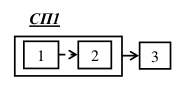
\includegraphics[resolution=128]{img/sd.png}

Заявки 1-го класса имеют относительный приоритет по отношению к заявкам 2-го
класса, по отношению к 3-ему классу заявки 1-го и 2-го имеют абсолютный приоритет.

\textbf{Дисциплина буферизации}

в) поступающая заявка любого класса при отсутствии свободного
места в накопителе данного класса теряется;

\textbf{Дисциплина прерывания}

а) прерванная заявка теряется;

\subsubsection{Параметры нагрузки}

\begin{tabular}{|c|c|c|c|c|c|}
\hline
\multicolumn{3}{|c|}{Интенсивность потока, $c^{-1}$} & \multicolumn{3}{c|}{Ср. длит. обслуживания, $c$} \\ \hline
$\lambda_1$      & $\lambda_2$     & $\lambda_3$     & $b_1$          & $b_2$          & $b_3$          \\ \hline
0,2              & 0,1             & 0,1             & 2,0            & 2,0            & 5,0            \\ \hline
\end{tabular}
\\

\subsection{Система}

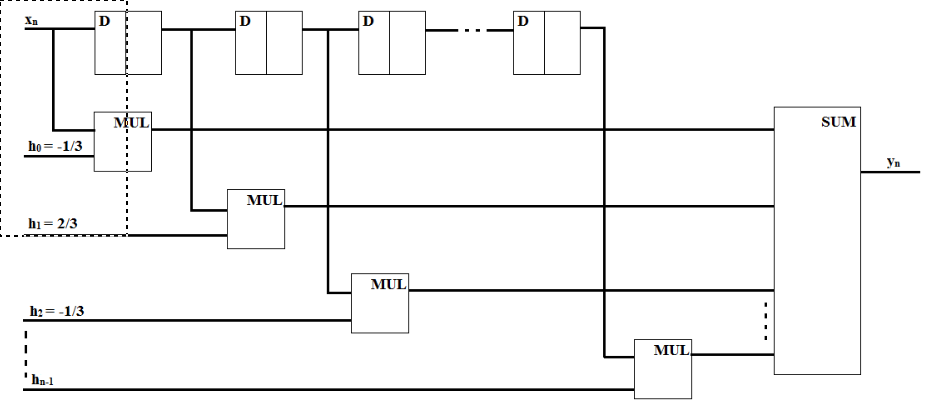
\includegraphics[resolution=128]{img/scheme.png}

\subsubsection{Перечень состояний}

\begin{tabular}{|c|c|}
\hline
Состояние & Код (Н1,Н2,Н3/П) \\ \hline
E0  & 0,0,0/0 \\ \hline
E1  & 0,0,0/1 \\ \hline
E2  & 0,0,0/2 \\ \hline
E3  & 0,0,0/3 \\ \hline
E4  & 0,0,1/1 \\ \hline
E5  & 0,1,0/1 \\ \hline
E6  & 0,1,1/1 \\ \hline
E7  & 1,0,0/1 \\ \hline
E8  & 1,0,1/1 \\ \hline
E9  & 1,1,0/1 \\ \hline
E10 & 1,1,1/1 \\ \hline
E11 & 0,0,1/2 \\ \hline
E12 & 0,1,0/2 \\ \hline
E13 & 0,1,1/2 \\ \hline
E14 & 1,0,0/2 \\ \hline
E15 & 1,0,1/2 \\ \hline
E16 & 1,1,0/2 \\ \hline
E17 & 1,1,1/2 \\ \hline
E18 & 0,0,1/3 \\ \hline
\end{tabular}

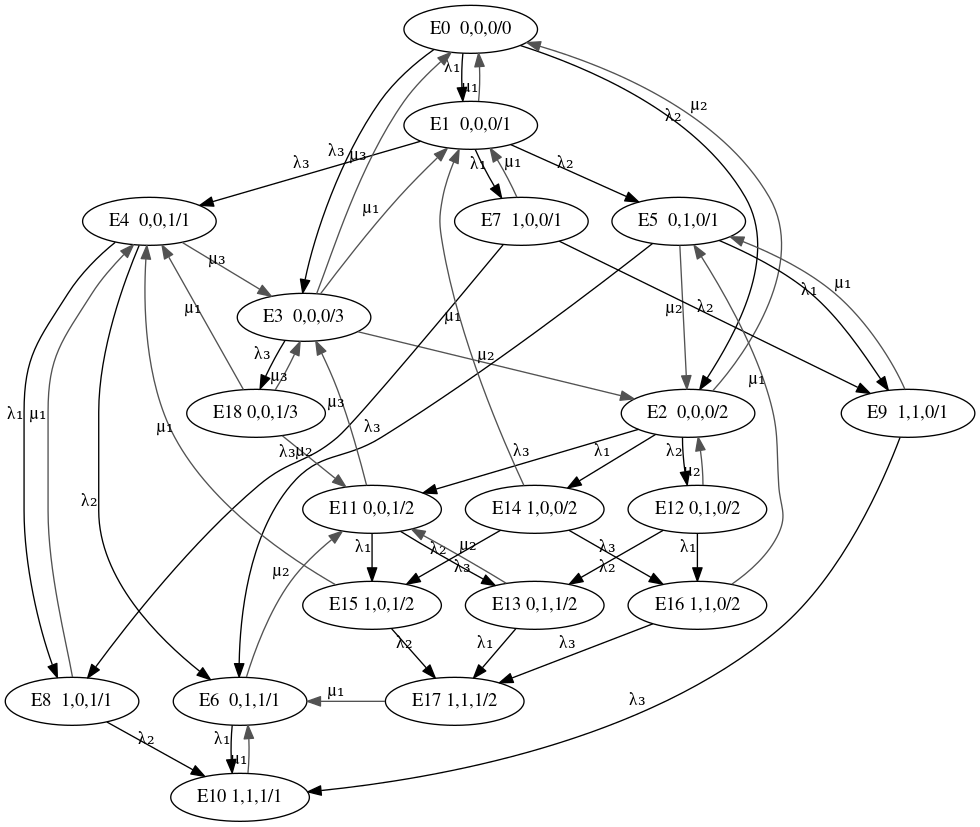
\includegraphics[width=\textwidth,height=\textheight,keepaspectratio]{img/graph.png}
\subsubsection{Матрица интенсивностей}

\begin{adjustbox}{max width=\textwidth}
\begin{tabular}{|c|c|c|c|c|c|c|c|c|c|c|c|c|c|c|c|c|c|c|c|}
\hline
  & 0 & 1 & 2 & 3 & 4 & 5 & 6 & 7 & 8 & 9 & 10 & 11 & 12 & 13 & 14 & 15 & 16 & 17 & 18 \\ \hline
0 & 1 & la2 & la3 & 0 & 0 & 0 & 0 & 0 & 0 & 0 & 0 & 0 & 0 & 0 & 0 & 0 & 0 & 0 \\ \hline
1 & mu1 & -0.9 & 0 & 0 & la3 & la2 & 0 & la1 & 0 & 0 & 0 & 0 & 0 & 0 & 0 & 0 & 0 & 0 & 0 \\ \hline
2 & mu2 & 0 & -0.9 & 0 & 0 & 0 & 0 & 0 & 0 & 0 & 0 & la3 & la2 & 0 & la1 & 0 & 0 & 0 & 0 \\ \hline
3 & mu3 & la1 & la2 & -0.6 & 0 & 0 & 0 & 0 & 0 & 0 & 0 & 0 & 0 & 0 & 0 & 0 & 0 & 0 & la3 \\ \hline
4 & 0 & 0 & 0 & mu1 & -0.8 & 0 & la2 & 0 & la1 & 0 & 0 & 0 & 0 & 0 & 0 & 0 & 0 & 0 & 0 \\ \hline
5 & 0 & 0 & mu1 & 0 & 0 & -0.8 & la3 & 0 & 0 & la1 & 0 & 0 & 0 & 0 & 0 & 0 & 0 & 0 & 0 \\ \hline
6 & 0 & 0 & 0 & 0 & 0 & 0 & -0.7 & 0 & 0 & 0 & la1 & mu1 & 0 & 0 & 0 & 0 & 0 & 0 & 0 \\ \hline
7 & 0 & mu1 & 0 & 0 & 0 & 0 & 0 & -0.7 & la3 & la2 & 0 & 0 & 0 & 0 & 0 & 0 & 0 & 0 & 0 \\ \hline
8 & 0 & 0 & 0 & 0 & mu1 & 0 & 0 & 0 & -0.6 & 0 & la2 & 0 & 0 & 0 & 0 & 0 & 0 & 0 & 0 \\ \hline
9 & 0 & 0 & 0 & 0 & 0 & mu1 & 0 & 0 & 0 & -0.6 & la3 & 0 & 0 & 0 & 0 & 0 & 0 & 0 & 0 \\ \hline
10 & 0 & 0 & 0 & 0 & 0 & 0 & mu1 & 0 & 0 & 0 & -0.5 & 0 & 0 & 0 & 0 & 0 & 0 & 0 & 0 \\ \hline
11 & 0 & 0 & 0 & mu2 & 0 & 0 & 0 & 0 & 0 & 0 & 0 & -0.8 & 0 & la2 & 0 & la1 & 0 & 0 & 0 \\ \hline
12 & 0 & 0 & mu2 & 0 & 0 & 0 & 0 & 0 & 0 & 0 & 0 & 0 & -0.8 & la3 & 0 & 0 & la1 & 0 & 0 \\ \hline
13 & 0 & 0 & 0 & 0 & 0 & 0 & 0 & 0 & 0 & 0 & 0 & mu2 & 0 & -0.7 & 0 & 0 & 0 & la1 & 0 \\ \hline
14 & 0 & mu2 & 0 & 0 & 0 & 0 & 0 & 0 & 0 & 0 & 0 & 0 & 0 & 0 & -0.7 & la3 & la2 & 0 & 0 \\ \hline
15 & 0 & 0 & 0 & 0 & mu2 & 0 & 0 & 0 & 0 & 0 & 0 & 0 & 0 & 0 & 0 & -0.6 & 0 & la2 & 0 \\ \hline
16 & 0 & 0 & 0 & 0 & 0 & mu2 & 0 & 0 & 0 & 0 & 0 & 0 & 0 & 0 & 0 & 0 & -0.6 & la3 & 0 \\ \hline
17 & 0 & 0 & 0 & 0 & 0 & 0 & mu2 & 0 & 0 & 0 & 0 & 0 & 0 & 0 & 0 & 0 & 0 & -0.5 & 0 \\ \hline
18 & 0 & 0 & 0 & mu3 & la1 & 0 & 0 & 0 & 0 & 0 & 0 & la2 & 0 & 0 & 0 & 0 & 0 & 0 & -0.5 \\ \hline

\end{tabular}
\end{adjustbox}

\subsubsection{Стационарные вероятности состояний}

\begin{tabular}{|l|l|}
\hline
Код состояния & Вероятность \\ \hline
E0 & 0.326416 \\ \hline
E1 & 0.134897 \\ \hline
E2 & 0.073543 \\ \hline
E3 & 0.131733 \\ \hline
E4 & 0.046789 \\ \hline
E5 & 0.031555 \\ \hline
E6 & 0.030392 \\ \hline
E7 & 0.038542 \\ \hline
E8 & 0.022020 \\ \hline
E9 & 0.016942 \\ \hline
E10 & 0.019949 \\ \hline
E11 & 0.035469 \\ \hline
E12 & 0.009193 \\ \hline
E13 & 0.006380 \\ \hline
E14 & 0.021012 \\ \hline
E15 & 0.015325 \\ \hline
E16 & 0.006566 \\ \hline
E17 & 0.006930 \\ \hline
E18 & 0.026347 \\ \hline
\end{tabular}

\subsubsection{Характеристики системы}
\begin{adjustbox}{max width=\textwidth}
\begin{tabular}{|c|c|c|c|}
\hline
Характеристика                      & Прибор & Расчетная формула                                                                                             & Значение  \\ \hline
\multirow{4}{*}{Нагрузка}           & П1     & $y_1 = \frac{\lambda_1}{\mu_1}$                                                                               & 0.400000  \\ \cline{2-4}
                                    & П2     & $y_2 = \frac{\lambda_2}{\mu_2}$                                                                               & 0.200000  \\ \cline{2-4}
                                    & П3     & $y_3 = \frac{\lambda_3}{\mu_3}$                                                                               & 0.500000  \\ \cline{2-4}
                                    & Сумма  & $y = y_1+y_2+y_3$                                                                                             & 1.100000  \\ \hline
\multirow{4}{*}{Загрузка}           & П1     & $\rho_1 = p_1+p_4+p_5+p_6+p_7+p_8+p_9+p_{10}$                                                                 & 0.341085  \\ \cline{2-4}
                                    & П2     & $\rho_2 = p_2+p_{11}+p_{12}+p_{13}+p_{14}+p_{15}+p_{16}+p_{17}$                                               & 0.174419  \\ \cline{2-4}
                                    & П3     & $\rho_3 = p_3+p_{18}$                                                                                         & 0.158080  \\ \cline{2-4}
                                    & Сумма  & $\rho = \rho_1+\rho_2+\rho_3$                                                                                 & 0.673584  \\ \hline
\multirow{4}{*}{Длина очереди}      & П1     & $l_1 = p_7+p_8+p_9+p_{10}+p_{14}+p_{15}+p_{16}+p_{17}$                                                        & 0.147287  \\ \cline{2-4}
                                    & П2     & $l_2 = p_5+p_6+p_9+p_{10}+p_{12}+p_{13}+p_{16}+p_{17}$                                                        & 0.127907  \\ \cline{2-4}
                                    & П3     & $l_3 = p_4+p_6+p_8+p_{10}+p_{11}+p_{13}+p_{15}+p_{17}+p_{18}$                                                 & 0.209601  \\ \cline{2-4}
                                    & Сумма  & $l = l_1+l_2+l_3$                                                                                             & 0.484795  \\ \hline
\multirow{4}{*}{Число заявок}       & П1     & $m_1 = l_1+\rho_1$                                                                                            & 0.488372  \\ \cline{2-4}
                                    & П2     & $m_2 = l_2+\rho_2$                                                                                            & 0.302326  \\ \cline{2-4}
                                    & П3     & $m_3 = l_3+\rho_3$                                                                                            & 0.367681  \\ \cline{2-4}
                                    & Сумма  & $m = l+\rho$                                                                                                  & 1.158378  \\ \hline
\multirow{4}{*}{Вероятность потери} & П1     & $\pi_1 = p_7+p_8+p_9+p_{10}+p_{14}+p_{15}+p_{16}+p_{17}$                                                      & 0.147287  \\ \cline{2-4}
                                    & П2     & $\pi_2 = p_5+p_6+p_9+p_{10}+p_{12}+p_{13}+p_{16}+p_{17}$                                                      & 0.127907  \\ \cline{2-4}
                                    & П3     & $\pi_3 = p_4+p_6+p_8+p_{10}+p_{11}+p_{13}+p_{15}+p_{17}+p_{18}$                                               & 0.209601  \\ \cline{2-4}
                                    & Сумма  & $\pi = \frac{(\lambda_1\cdot\pi_1+\lambda_2\cdot\pi_2+\lambda_3\cdot\pi_3)}{(\lambda_1+\lambda_2+\lambda_3)}$ & 0.158020  \\ \hline
\multirow{4}{*}{Производительность} & П1     & $\lambda'_1 = \lambda_1\cdot (1-\pi_1)$                                                                       & 0.170543  \\ \cline{2-4}
                                    & П2     & $\lambda'_2 = \lambda_2\cdot (1-\pi_2)$                                                                       & 0.087209  \\ \cline{2-4}
                                    & П3     & $\lambda'_3 = \lambda_3\cdot (1-\pi_3)$                                                                       & 0.079040  \\ \cline{2-4}
                                    & Сумма  & $\lambda' = \lambda'_1+\lambda'_2+\lambda'_3$                                                                 & 0.336792  \\ \hline
\multirow{4}{*}{Время ожидания}     & П1     & $\omega_1 = \frac{l_1}{\lambda'_1}$                                                                           & 0.863636  \\ \cline{2-4}
                                    & П2     & $\omega_2 = \frac{l_2}{\lambda'_2}$                                                                           & 1.466666  \\ \cline{2-4}
                                    & П3     & $\omega_3 = \frac{l_3}{\lambda'_3}$                                                                           & 2.651834  \\ \cline{2-4}
                                    & Сумма  & $\omega = \frac{l}{\lambda'}$                                                                                 & 1.439448  \\ \hline
\multirow{4}{*}{Время пребывания}   & П1     & $u_1 = \frac{m_1}{\lambda'_1}$                                                                                & 2.863636  \\ \cline{2-4}
                                    & П2     & $u_2 = \frac{m_2}{\lambda'_2}$                                                                                & 3.466666  \\ \cline{2-4}
                                    & П3     & $u_3 = \frac{m_3}{\lambda'_3}$                                                                                & 4.651834  \\ \cline{2-4}
                                    & Сумма  & $u = \frac{m}{\lambda'}$                                                                                      & 3.439449  \\ \hline
\end{tabular}
\end{adjustbox}

\subsubsection{Графики варьирования}
\subsubsubsection{По интенсивности потоков заявок}
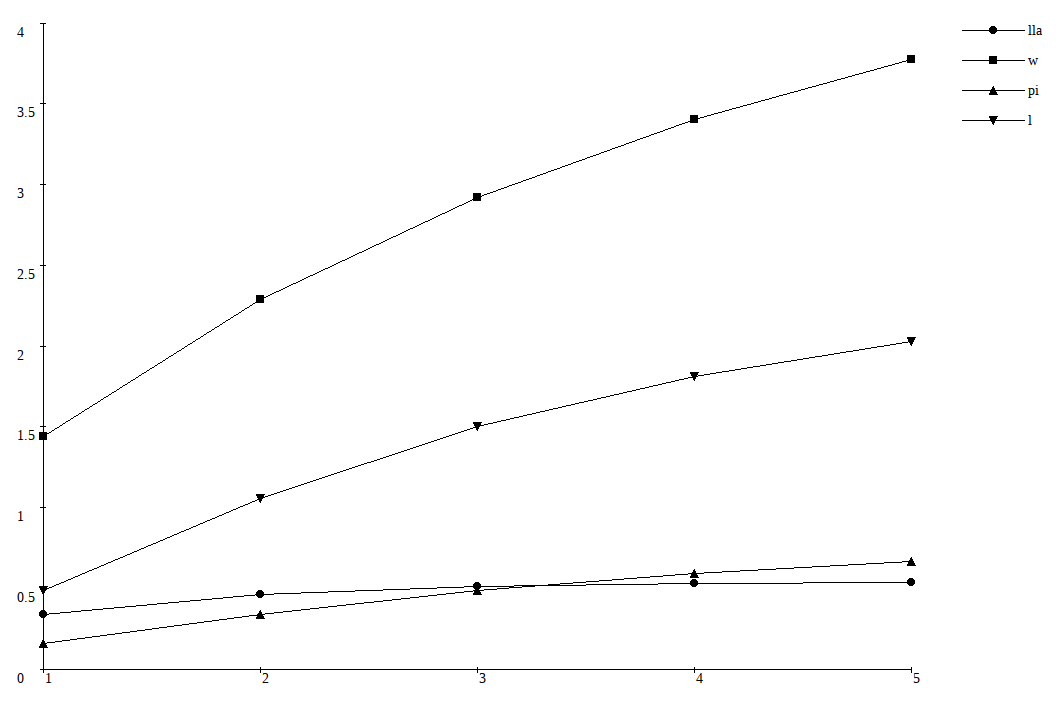
\includegraphics[width=\textwidth,height=\textheight,keepaspectratio]{img/lagraph.png}

\subsubsubsection{По средней интенсивности обслуживания}
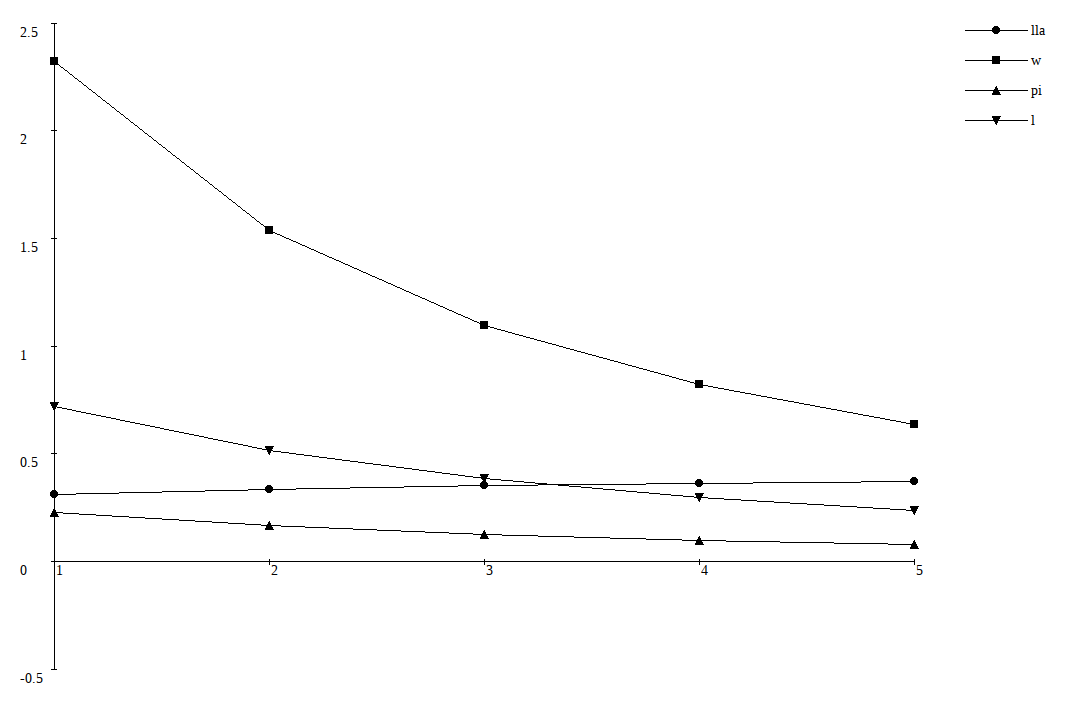
\includegraphics[width=\textwidth,height=\textheight,keepaspectratio]{img/mugraph.png}
\section{Вывод}
Исходя из полученных данных можно проследить зависимость между средней интенсивностью потока
заявок или обслуживанию и всеми остальными параметрами: для интенсивности потока заявок данная
зависимость прямо пропорциональная, и обратно пропорциональная для интенсивности обслуживания.
\end{document}
